% ----------------------------------------------------------------------------
\section{Projektmanagement}
\begin{frame}[fragile]
	\frametitle{Projektmanagement}
\huge Projektmanagement
\end{frame}

\begin{frame}
\frametitle{Erfolgskriterien}
	Es gibt einige, allgemeine Erfolgskriterien die alle Projekte teilen
	\begin{itemize}
		\item Software wird innerhalb der definierten Zeit fertiggestellt
		\item Kosten liegen innerhalb der Budgetplanung
		\item Gelieferte Software entspricht der Erwartung des Kunden
		\item Entwicklungsteam arbeitet kohärent und effizient zusammen
	\end{itemize}
\end{frame}

\begin{frame}
\frametitle{Charakteristika von Softwareprojekten}
	Softwareprojekte haben bestimmte Charakteristika die sie von Projekten
	in anderen Bereichen unterscheiden
	\begin{itemize}
		\item Software ist intangibel
		\item Große SW-Projekte sind in Technologie, Vorgehen, Organisation
		einzigartig
		\item Prozesse und Vorgehensmodelle sind flexibel und organisationsspezifisch
	\end{itemize}
\end{frame}

\begin{frame}
\frametitle{Managementfaktoren in SW-Projekten}
	\begin{itemize}
		\item Größe der Organisation
		\item Kundentyp
		\item Komplexität der Software
		\item Softwaretyp
		\item Unternehmenskultur
		\item Softwareentwicklungsprozesse
	\end{itemize}
\end{frame}

\begin{frame}
\frametitle{Fundamentale PM Aktivitäten}
	\begin{enumerate}
		\item Projektplanung
		\item Risikomanagement
		\item Personalführung
		\item Berichterstattung
		\item Projektierung
	\end{enumerate}
\end{frame}

\subsection{Risikomanagement}
\begin{frame}
\frametitle{Risikomangement}
\huge Risikomangement
\end{frame}

\begin{frame}
\frametitle{Risikomanagement}
	\begin{block}{Risiko}
		Ein Problem, das noch nicht eingetreten ist, aber wichtige Projektziele
		oder Projektergebnisse gefährdet, falls es eintritt. Ob es eintreten wird
		kann nicht sicher vorausgesagt werden.
	\end{block}
	\begin{itemize}
		\item In jedem Projekt treten Probleme auf die die Projektziele gefährden
		\item Risikomanagement versucht mögliche Probleme frühzeitig zu identifizieren
		und Maßnahmen einzuleiten
		\item Risikomanagement ist eine kontinuierliche Aktivität und umfasst
		\begin{itemize}
			\item Identifikation von Risiken
			\item Analyse und Bewertung der Risiken
			\item Planung von Gegenmaßnahmen
			\item Risikoüberwachung
		\end{itemize}
	\end{itemize}
\end{frame}

\begin{frame}
\frametitle{Identifikation von Risiken}
	Eine Risikoeinordnung kann sein
	\begin{itemize}
		\item Projektrisiken die den Projektplan oder -ressourcen beeinflussen
		\item Produktrisiken die Qualität oder Effizienz der Applikation mindern
		\item Geschäftsrisiken den zugrundeliegenden Business Plan der Applikation beeinflussen
	\end{itemize}
\end{frame}

\begin{frame}
\frametitle{Identifikation von Risiken}
	\begin{itemize}
		\item Es kann auch zwischen Kernrisiken und projektspezifischen Risiken unterschieden werden.
		\item Projektspezifischre Risiken können beispielsweise im Rahmen eines moderierten
		Workshops erhoben werden
	\end{itemize}
\end{frame}

\begin{frame}
\frametitle{Übung 3.1}
	Überlegen Sie, welche Kernrisiken für einen Großteil der Soll-Ist-Abweichungen
	in Softwareprojekten verantwortlich ist.
\end{frame}

\ifloesung
\begin{frame}
\frametitle{Übung 3.1 - Lösung}
	\begin{itemize}
		\item Unklare bzw. sich laufend ändernde Projektziele und Anforderungen
					die grundlegende Änderungen am Quellcode erfordern
		\item Unkorrekter Zeitpland, z.B. die
					Dauer der Testphase wurde unterschätzt oder gar unterschlagen
		\item Mitarbeiterfluktuation im Projektteam
		\item Mangelnde Skills der Mitarbeiter
		\item Fehlende Unterstützung im Management
		\item Organisatorische Änderungen wie beispielsweise wechselnde Projektverantwortliche
		\item Grundlegend falsch gewählte Technologien
		\item \ldots
	\end{itemize}
\end{frame}
\fi

\begin{frame}
\frametitle{Analyse und Bewertung von Risiken}
	\begin{block}{Risikowert}
		Risikowert = p * K
		\begin{itemize}
			\item p = Eintrittswahrscheinlichkeit
			\item K = Kosten die im Schadensfall enstehen
		\end{itemize}
	\end{block}
	\begin{itemize}
		\item Risiken mit p \textgreater 0.5 sollten als sicheres Ereignis angesehen werden
		\item Jeder Risikowert kann als Punkt in einem Risikodiagramm eingesetzt werden
		\item Ein Risikodiagramm besitzt auf beiden Achsen eine logarithmische Skalierung
		\item Kleine Risikowerte müssen nicht Kontrolliert werden
	\end{itemize}
\end{frame}

\begin{frame}
\frametitle{Risikodiagramm}
	Das dargestellte Risikodiagramm bewertet Risikowerte bis 10000 Euro als akzeptabel
	\center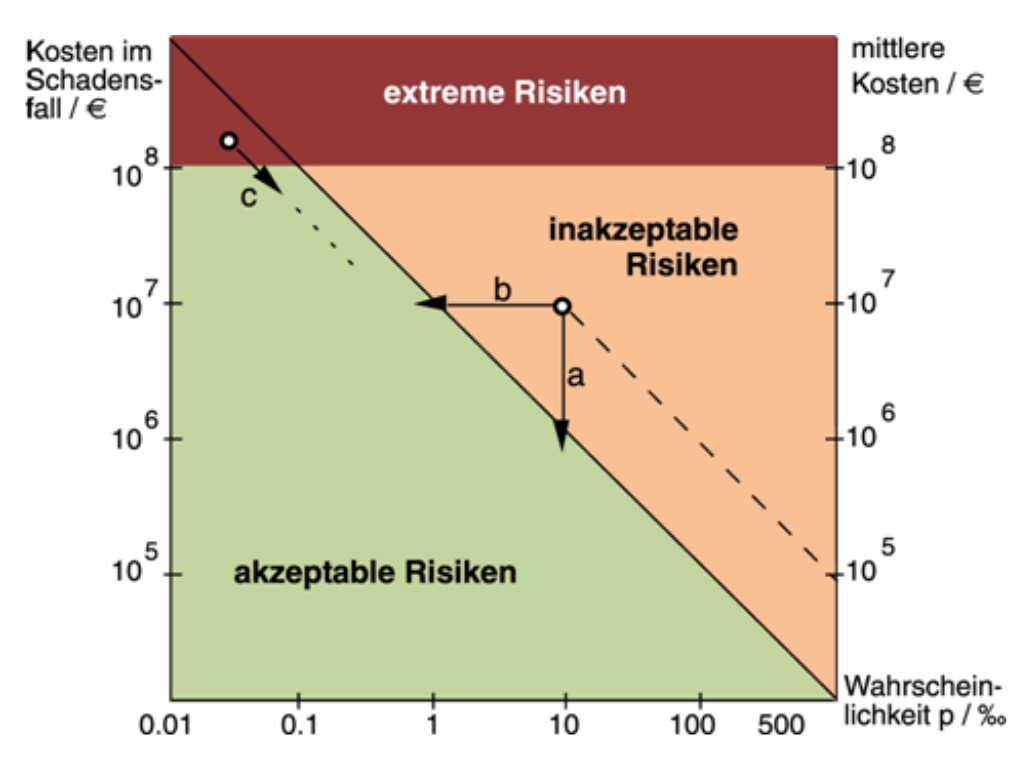
\includegraphics[width=1\textwidth,
		keepaspectratio=true]{bilder/risikodiagramm.png}
\end{frame}

\begin{frame}
\frametitle{Risikodiagramm}
	\begin{itemize}
		\item Für Punkte unter der Diagonalen sind keine Aktionen erforderlich
		\item Punkte über der Diagonalen müssen nach links oder unten verschoben werden
		\item Senkung der Kosten bei Risikoeintritt verschiebt den Punkt nach unten (Pfeil a)
		\item Senkung der Wahrscheinlichkeit verschiebt den Punkt nach links (Pfeil b)
		\item Alle Maßnahmen führen zu zusätzlichen sicheren Kosten die deutlich geringer sind
					als der mögliche Schaden
		\item Oben liegen extreme Risiken deren Schaden nicht beherrschbar ist (z.B. Firmenbankrott)
		\item Bei einem solchen Extremrisiko kann eine Versicherung in Erwägung gezogen werden die aus
					großem Eintrittschaden eine kleinere sichere Zahlung macht (Pfeil c)
	\end{itemize}
\end{frame}

\begin{frame}
\frametitle{Risikomatrix}
	Alternativ kann man mit einer diskreten Bewertung arbeiten
		\begin{table}[]
			\begin{tabular}{ll}
			 Wert (p) & Eintrittswahrscheinlichkeit \\
			 \hline
			 1 & Unwahrscheinlich \\
			 2 & Denkbar \\
			 3 & Wahrscheinlich \\
			 	 &	\\
			 Wert (k) & Schadensausmaß \\
			 \hline
			 1 & Gering \\
			 2 & Beträchtlich \\
			 3 & Groß
			\end{tabular}
		\end{table}
\end{frame}

\begin{frame}
\frametitle{Risikomatrix}
	Die Risiken können entsprechend klassifiziert werden um daraus eine Risikomatrix
	abzuleiten.
	\bigskip
	\begin{small}
		\begin{table}[]
			\begin{tabular}{l|lll}
			 Groß 				& \cellcolor[HTML]{FFCD69} 3 & \cellcolor[HTML]{FC6D58} 6 & \cellcolor[HTML]{D8334A} 9 \\
			 Beträchtlich & \cellcolor[HTML]{E8CE4D} 2 & \cellcolor[HTML]{F39C12} 4 & \cellcolor[HTML]{FC6D58} 6 \\
			 Gering 			& \cellcolor[HTML]{9FD477} 1 & \cellcolor[HTML]{E8CE4D} 2 & \cellcolor[HTML]{FFCD69} 3 \\
			 \hline
			 							& Unwahrscheinlich  				 & Denkbar 										& Wahrscheinlich
			\end{tabular}
		\end{table}
	\end{small}
	\bigskip
	Auch hier ist zu bestimmen welche Risikowerte kontrolliert werden müssen.
\end{frame}

\begin{frame}
\frametitle{Gegenmaßnahmen}
	\begin{itemize}
		\item Zur Risikobegrenzung sollten Zeit-/Geldreservern eingeplant werden
		\item Die Rückstellung sollte dem Risikowert entsprechen
		\item Präventivmaßnahmen sind aktiv
					\begin{itemize}
						\item Senken der Eintrittswahrscheinlichkeit
						\item Schaden auf eine vertretbae Höhe beschränken
					\end{itemize}
		\item Notfallmaßnahmen im Schadensfall sind reaktiv
		\item Präventive und reaktive Maßnahmen müssen im Projektplan berücksichtigt werden
	\end{itemize}
\end{frame}

\begin{frame}
\frametitle{Übung 3.2}
	In ihrem Projekt haben Sie den weggang eines wichtigen Mitarbeiters als Risiko identifiziert.
	Nennen Sie eine Präventivmaßnahme, um die Eintrittswahrscheinlichkeit dieses Risikos zu senken
	sowie eine Präventivmaßnahme um die Höhe des Schadens zu senken. Was ist eine mögliche
	Notfallmaßnahme?
\end{frame}

\ifloesung
\begin{frame}
\frametitle{Übung 3.2 - Lösung}
	Eintrittswahrscheinlichkeit senken:
	\begin{itemize}
		\item Horizontale/Vertikale Karriereanreiz schaffen
	\end{itemize}

	Schaden senken:
	\begin{itemize}
		\item Wissensmanagement/Projektkonzept für schnelle Einarbeitung etablieren
	\end{itemize}

	Notfallmaßnahme:
	\begin{itemize}
		\item Projektscope verkleinern
	\end{itemize}
\end{frame}
\fi

\begin{frame}
\frametitle{Risikoüberwachung}
	\begin{itemize}
		\item Risiken ändern sich während des Projektverlaufs
					\begin{itemize}
						\item Schwächen ab
						\item Verstärken sich
						\item Sind nicht mehr existent
						\item Entstehen
					\end{itemize}
		\item Risikosituation musst stetig neu bewertet werden
		\item Regelmäßige Projektsitzungen sind unabdinglich
		\item Risiken müssen offen kommuniziert werden dürfen
	\end{itemize}
\end{frame}

\subsection{Qualitätssicherung}
\begin{frame}
\frametitle{Qualitätssicherung}
\huge Qualitätssicherung
\end{frame}

\begin{frame}
\frametitle{Qualitätssicherung}
	\begin{block}{Qualität}
		Gesamtheit von Eigenschaften und Merkmalen eines Produktes oder einer Tätigkeit,
		die sich auf die Eignung zur Erfüllung gegebener Erfordernisse beziehen.
	\end{block}
	\begin{itemize}
		\item Im Software Engineering gibt es zwei Sichtweisen auf die Qualität
		\begin{itemize}
			\item Prozessqualität (z.B. bewertbar durch CMMI)
			\item Produktqualität
		\end{itemize}
		\item Produktqualität umfasst Wartbarkeit und Brauchbarkeit
		\item Geforderte Qualitätsanforderungen müssen definiert und die Einhaltung
					dieser Anforderungen geprüft werden
	\end{itemize}
\end{frame}

\begin{frame}
\frametitle{Qualitätssicherung}
	\begin{block}{Qualitätsmanagement}
		Aufeinander abgestimmte Tätigkeiten zum Leiten und Lenken einer Organisation
		bezüglich Qualität, die üblicherweise das festlegen der Qualitätspolitik und
		-ziele, die -planung, die -lenkung die -sicherung und die Qualitätsverbesserung
		umfassen.
	\end{block}
	\begin{itemize}
		\item Unter Qualitätsmanagement werden die managementbezogenen Tätigkeiten zusammengefasst
		\item Unter Qualitätssicherung werden die technisch orientierten Aktivitäten zusammengefasst
	\end{itemize}
\end{frame}

\begin{frame}
\frametitle{Qualitätssicherung}
	Es werden drei Maßnahmen zur Qualitätssicherung unterschieden
	\begin{itemize}
		\item Organisatorische Maßnahmen
					\begin{itemize}
						\item Systematische Entwicklung und QS
						\item Zeitplanung für Testing und Bugfixing
						\item Rollen / Verantwortlichkeiten für QS
						\item Vorgabe von Richtlinien, Standards, Checklisten
					\end{itemize}
		\item Konstruktive Maßnahmen
					\begin{itemize}
						\item Fehler und schlechte Qualität von Beginn an vermeiden
						\item ``Es kann keine Qualität in ein Produkt hineingeprüft werden''
					\end{itemize}
		\item Analytische Maßnahmen
					\begin{itemize}
						\item Software-Tests
						\item Metriken
						\item Audits
						\item Fehler und Mängel in den Arbeitsergebnissen erkennen
					\end{itemize}
	\end{itemize}
	Organisatorische und konstruktive Maßnahmen sind hilfreicher als analytische Maßnahmen.
\end{frame}

\begin{frame}
\frametitle{Übung 3.3}
	Nennen Sie konstruktive Maßnahmen die dabei helfen Mängeln bei der Software-Entwicklung aus dem
	Weg zu gehen.
\end{frame}

\ifloesung
\begin{frame}
\frametitle{Übung 3.3 - Lösung}
	\begin{itemize}
		\item Passendes und vor allem korrekt eingesetztes Vorgehensmodell definieren
		\item Eingeplante Code-Reviews
		\item Pair-Programming
		\item Definierte Quality Gates mit klaren abnahmekriterien
		\item Einführung von Continuous Integration und Continuous Deployment
		\item Verwendung von typisierter Programmiersprache
		\item Schulungen
		\item Konfigurationsmanagement
		\item Passende Werkzeuge/Methoden etablieren
		\item \ldots
	\end{itemize}
\end{frame}
\fi

\begin{frame}
\frametitle{Qualitätssicherung}
	\begin{itemize}
		\item Fehler die früh in der Entwicklung entstehen und unentdeckt bleiben können zu Summationseffekten
		in späteren Phasen führen
		\item Folgende Ziele sollten verfolgt werden:
					\begin{itemize}
						\item Kein Fehler machen (z.B. durch konstruktive Maßnahmen)
						\item Fehler die dennoch gemacht wurden möglichst früh entdecken und beseitigen
					\end{itemize}
	\end{itemize}
\end{frame}

\begin{frame}
\frametitle{Übung 3.4}
	Es wird ein Software-Test vorgenommen. Ist es ratsam, jeden entdeckten Fehler sofort zu
	korrigieren oder gibt es Gründe die Korrektur von der Prüfung zu trennen?
\end{frame}

\ifloesung
\begin{frame}
\frametitle{Übung 3.4 - Lösung}
	\begin{itemize}
		\item Korrektur ist Änderung des Artifakts und bedarf eines erneuten Deployments
		\item Korrektor kann langwierig sein (von wenigen Minuten bis zu mehreren Tagen)
		\item Einfache Fehler mit geringen Effekten haben ggf. weniger Priorität
		\item \ldots
	\end{itemize}
	Es sollte stehts zwischen Test und Korrektur getrennt werden.
\end{frame}
\fi

\begin{frame}
\frametitle{Agiles Qualitätsmanagement}
	\begin{itemize}
		\item Qualität in der agilen Softwareentwicklung bedeutet Codequalität
		\item Fokus liegt auf Praktiken wie Refactoring und testgetriebener Entwicklung
		\item QM ist formlos und basiert auf qualitätsgetriebener Projektkultur
		\item Jedes Teammitglied ist für SW-Qualität im Projekt verantwortlich
	\end{itemize}
\end{frame}

\begin{frame}
\frametitle{Good practices im agilen Qualitätsmanagement}
	\begin{itemize}
		\item Check before check-in \\
				  Entwickler organisieren selbst Code-Review bevor Code gemerged wird
		\item Never break the build \\
		 			Es wird kein Code gepushed der das System als Ganzes zerstört. Wer einen
					fehlerhaften Build pushed muss die Probleme mit höchster Priorität beheben
		\item Fix problems when you see them \\
		 			Der Code des Systems gehört dem ganzen Team. Findet ein Entwickler einen Fehler
					kann er ihn selbst beheben ohne auf den Autor verweisen zu müssen.
	\end{itemize}
\end{frame}

\begin{frame}
\frametitle{Good practices im agilen Qualitätsmanagement}
	\begin{itemize}
		\item Testgetriebene Entwicklung \\
					Test first programming. Es wird zuerst der Testfall geschrieben und im Anschluss
					gegen ihn entwickelt
		\item Continuous Integration
					Kontinuierliche Integration von Codeänderungen mit anschließender Verfikikation
					durch Bau des Artefakts
		\item Continuous Delivery
					Möglichkeit kontinuierlich Codeänderungen auf QA/Produktionssysteme in Betrieb
					nehmen zu können
	\end{itemize}
\end{frame}

\begin{frame}
\frametitle{Grundvoraussetzungen für agiles Qualitätsmanagement}
	\center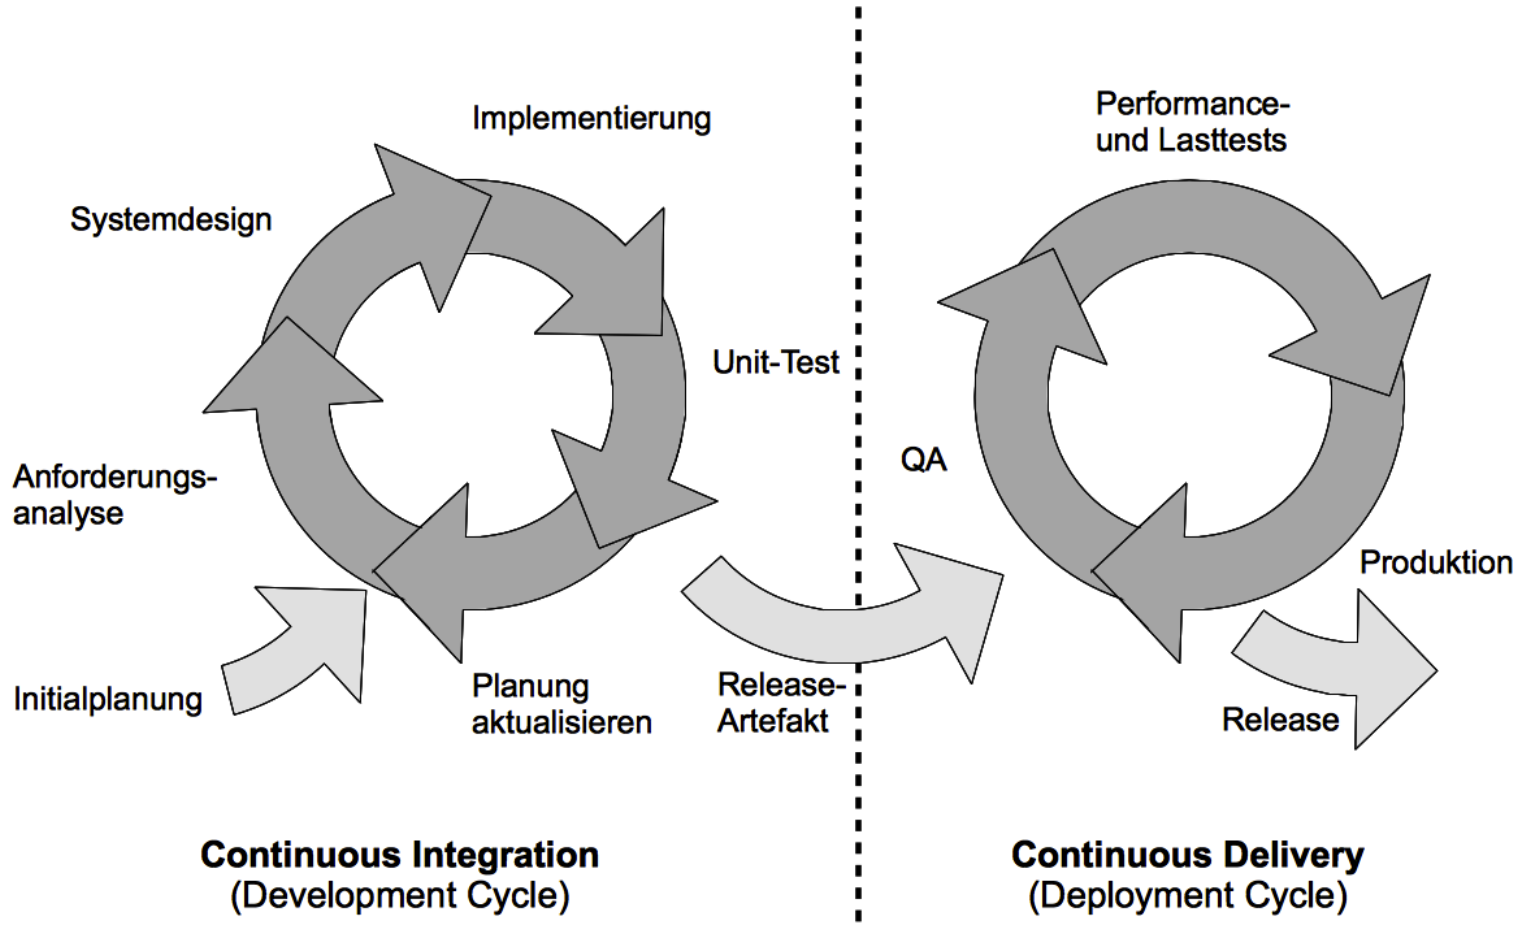
\includegraphics[width=1\textwidth,
		keepaspectratio=true]{bilder/continuous_delivery.png}
\end{frame}

\begin{frame}
\frametitle{Test-Pyramide}
	\center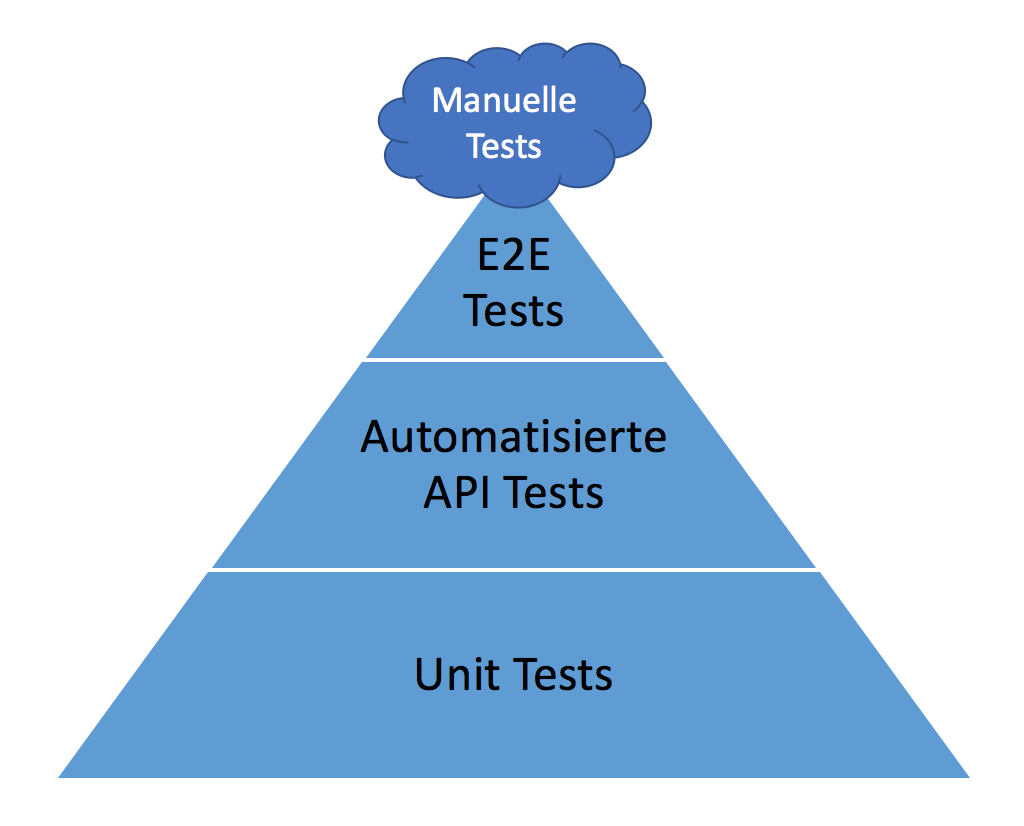
\includegraphics[width=1\textwidth,
		keepaspectratio=true]{bilder/test_pyramide.png}
	\end{frame}

\begin{frame}
\frametitle{Test-Eiswaffel}
	\center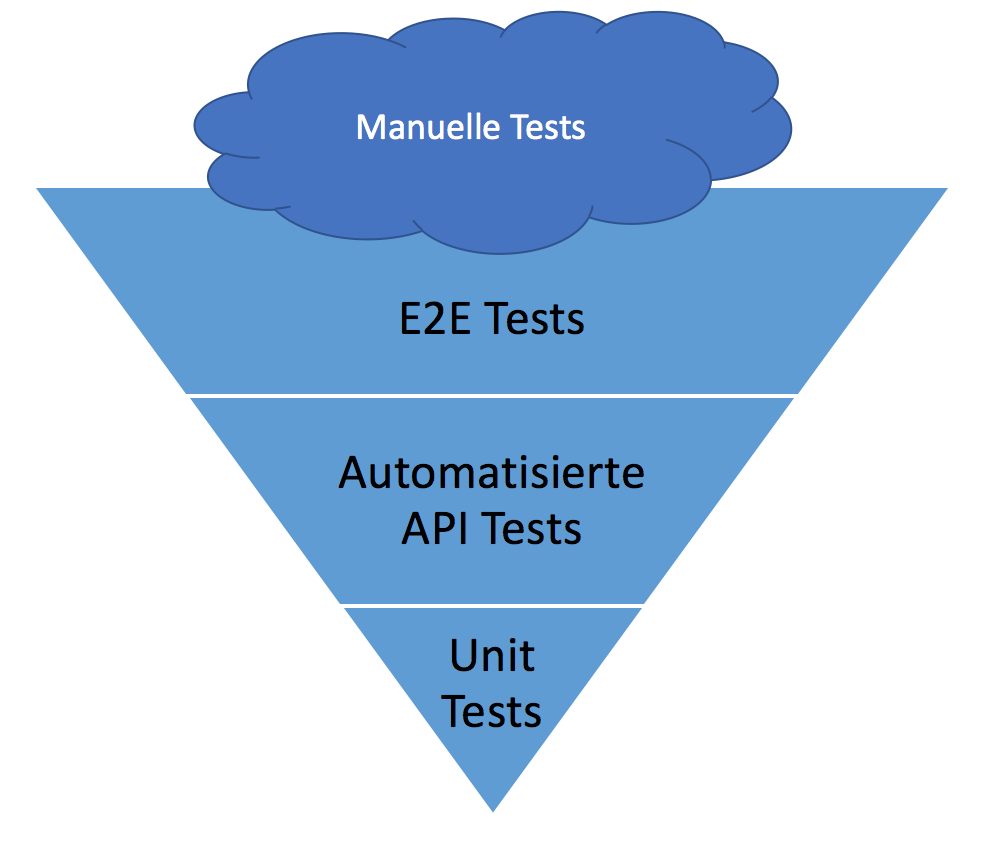
\includegraphics[width=1\textwidth,
		keepaspectratio=true]{bilder/test_eiswaffel.png}
\end{frame}

\begin{frame}
\frametitle{Programmtest}
	\begin{itemize}
		\item Weist fehlerfreiheit des Software-Systems nach
		\item Aufgrund der hohen Komplexität ist Nachweis von Fehlerfreiheit unmöglich
		\item Ziel des Testens ist es daher möglichst viele vorhandene Fehler zu finden
		\item Konkretes Programm wird dazu ausgeführt und mit Werten gefüttert
		\item Ist-Werte werden mit den Soll-Werten aus der Spezifikation verglichen
		\item Bei Abweichung zwischen Ist-Wert und Soll-Wert liegt ein Fehler vor
	\end{itemize}
\end{frame}

\begin{frame}
\frametitle{Programmtest}
	Systematische Tests
	\begin{itemize}
		\item Randbedingungen (z.B. Systemumgebung) ist definiert
		\item Eingaben werden systematisch ausgewählt
		\item Soll-Werte werden vor dem Test festgelegt
		\item Gesamter Test wird dokumentiert
		\item Test und Korrektur finden getrennt statt
	\end{itemize}
	Systematische Tests sind stets reproduzierbar und damit objektiv und wiederholbar.
\end{frame}

\begin{frame}
\frametitle{Programmtest}
	Es können verschiedene Eigenschaften eines Programms getestet werden woraus sich folgende
	Testklassifikation ergibt
	\begin{itemize}
		\item Funktionstest
		\item Last- und Stresstest
		\item Verfügbarkeitstest
		\item Installationstest
		\item Wiederinbetriebnahmetest
	\end{itemize}
	Mindestens Funktions- oder Lasttests sollten systematisch durchgeführt werden.
\end{frame}

\begin{frame}
\frametitle{Programmtest}
	\begin{itemize}
		\item Ein vollständiger Test deckt alle möglichen Eingaben für ein Programm ab
		\item Ist ein vollständiger Test fehlerfrei wurde die Korrektheit des Programms bewiesen
		\item Bereits für einfache Funktion mit ganzahligem Parameter ergibt dies 2\textsuperscript{32} Möglichkeiten
		\item Aus diesem Grund wird Teilmenge getestet und die Eingaben werden geeignet gewählt
	\end{itemize}
\end{frame}

\begin{frame}
\frametitle{Black-Box Test}
	\begin{block}{Black-Box Test}
		Testfälle werden auf Basis der in der Spezifikation geforderten Eigenschaften gewählt.
		Die innere Beschaffenheit des Programms spielt keine Rolle.
	\end{block}
	\begin{itemize}
		\item Testfälle werden aufgestellt sobald die Spezifikation vorliegt
		\item Folgende Verfahren werden zur Bestimmung der Testfälle betrachtet:
			\begin{itemize}
				\item Funktionale Äquivalenzklassenbildung
				\item Grenzwertanalyse
				\item Test spezieller Werte
				\item Zufallstest
			\end{itemize}
	\end{itemize}
\end{frame}

\begin{frame}
\frametitle{Funktionale Äquivalenzklassenbildung}
	\begin{itemize}
		\item Angenommen es existiert eine Menge E = {e1, e2, ..., en} von Eingaben auf die das
					das Programm identisch reagiert
		\item Dann reicht es aus lediglich eine Eingabe dieser Menge zu testen
		\item Wenn die Eingabe fehlerfrei ist kann man von Korrektheit der restlichen Eingaben ausgehen
		\item Eine solche Menge wird als Äquivalenzklasse bezeichnet
		\item Jede Eingabe aus der Äquivalenzklasse ist damit repräsentativ für jede andere Eingabe
					der Äquivalenzklasse
		\item In der Praxis wird häufig nur vermutet das Eingaben Äquivalent, dann wird auch von
					schwacher Äquivalenz gesprochen
	\end{itemize}
\end{frame}

\begin{frame}
\frametitle{Vorgehen bei Äquivalenzklassentest}
	\begin{enumerate}
		\item Menge der Eingaben wird in Äquivalenzklassen zerlegt
		\item Testfälle werden aus Eingaben aus möglichst vielen Äquivalenzklassen zusammengestellt
		\item Ein Testfall sollte höchstens nur eine Eingabe aus einer ungültigen Äquivalenzklasse
					enthalten um die Fehlerbehandlung klar identifizieren zu können
	\end{enumerate}
\end{frame}

\begin{frame}
\frametitle{Grenzwertanalyse}
	\begin{itemize}
		\item Besitzen die Äquivalenzklassen eine natürliche Ordnung werden die Elemente der Klasse
					gewählt die an den Grenzen liegen
		\item Annäherung an die Grenzen kann vom gültigen und vom ungültigen Bereich der Klasse erfolgen
	\end{itemize}
\end{frame}

\begin{frame}
\frametitle{Test spezieller Werte}
	\begin{itemize}
		\item Bei zunehmender Testerfahrung werden Eingaben identifiziert die fehleranfälliger sind
					als andere
		\item Diese Eingaben werden für spätere Testfälle dokumentiert
		\item Beispiele: leere Eingabe, Sonderzeichen
	\end{itemize}
\end{frame}

\begin{frame}
\frametitle{Zufallstest}
	\begin{itemize}
		\item Testfälle werden zufällig generiert
		\item Datentypen und Struktur der Eingaben müssen bei Generierung berücksichtigt werden
		\item Ist ein ergänzendes Verfahren
		\item Deckt auch nicht naheliegene Eingaben ab
	\end{itemize}
\end{frame}

\begin{frame}
\frametitle{White-Box Test}
	\begin{block}{White-Box Test}
		Der Programmcode ist sichtbar. Es wird ein Strukturtest vorgenommen. Dabei wird die
		überdeckung des Codes durch die Testfälle analysiert. Das Ziel ist es eine vorgegebene
		Überdeckungsrate zu erreichen.
	\end{block}
	\begin{itemize}
		\item Um die Überdeckungsrate bestimmen zu können muss das Programm mit zusätzlichen
					Anweisungen für die Messung instrumentiert werden
		\item Dadurch kann z.B. gezählt werden wie häufig eine Programmzeile ausgeführt wurde
		\item Es werden verschiedene Überdeckungskriterien unterschieden
					\begin{itemize}
						\item Anweisungsüberdeckung
						\item Zweigüberdeckung
						\item Bedingungsüberdeckung
					\end{itemize}
	\end{itemize}
\end{frame}

\subsection{Messen/Bewerten}
\begin{frame}
\frametitle{Messen und Bewerten}
\huge Messen und Bewerten
\end{frame}

\begin{frame}
\frametitle{Projekt-Controlling}
	\begin{itemize}
		\item Während des Projektverlaufs muss der Projektfortschritt durchgehend kontrolliert
					und gesteuert werden
		\item Dabei müssen folgende Tätigkeiten ausgeführt werden
					\begin{enumerate}
						\item Das Soll ermitteln
						\item Das Ist ermitteln
						\item Soll-Ist-Vergleich
						\item Bei Abweichung korrigierende Maßnahmen einrichten
					\end{enumerate}
		\item Projekt-Controlling setzt voraus dass bereits geleistete Arbeitsstunden erfasst wurden
		\item Arbeitsstunden der Mitarbeiter werden jeweiligen Arbeitspaketen zugeordnet
		\item Ist-Wert kann mit geplanten Soll-Wert (Aufwandsschätzung) verglichen werden
	\end{itemize}
\end{frame}

\begin{frame}
\frametitle{Übung 3.5}
	Wann entstehen Abweichungen zwischen dem Ist-Aufwand und dem geplanten Soll-Aufwand für ein
	Arbeitspaket?
\end{frame}

\ifloesung
\begin{frame}
\frametitle{Übung 3.5 - Lösung}
	\begin{itemize}
		\item Mangelnde technische Kenntnisse
		\item Externe Abhängikeiten die zu Verzögerung führen
		\item Aufwand für noch zu erledigende Leistungen wird unterschätzt
		\item Erbrachte Leistung wurde überschätzt
		\item \ldots
	\end{itemize}
\end{frame}
\fi

\begin{frame}
\frametitle{Projekt-Controlling - Fertigstellungsgrad}
	\begin{block}{Fertigstellungsgrad 1}
		FG1 = Ist-Aufwand / Geschätzter Gesamtaufwand
	\end{block}
	Selbst wenn die Schätzung des Gesamtaufwands gut ist, wird FG1 am Ende des Projektes ungenau.
	Daher ist es besser eine transparentere Aufwandsschätzung zu verwenden, die den geschätzten
	Restaufwand miteinbezieht.
	\begin{block}{Fertigstellungsgrad 2}
		FG2 = Ist-Aufwand / (Ist-Aufwand + Geschätzter Restaufwand)
	\end{block}
\end{frame}

\begin{frame}
\frametitle{Projekt-Controlling - Fertigstellungsgrad}
	Ist es aus organisatorischen Gründen nicht möglich den Ist-Aufwand zeitnah zur
	Verfügung zu stellen kann man den erarbeiteten Wert verwenden.
	\begin{block}{Erarbeiteter Wert}
		EW = Geplanter Aufwand - Restaufwand
	\end{block}
	Daraus ergibt sich der Fertigstellungsgrad 3.
	\begin{block}{Fertigstellungsgrad 3}
		FG3 = EW / Geplanter Aufwand
	\end{block}
\end{frame}

\begin{frame}
\frametitle{Projekt-Controlling - Fertigstellungsgrad}
	Der Fertigstellungsgrad kann auch auf Grundlage der bereits abgeschlossenen Arbeitspakete
	berechnet werden.
	\begin{block}{Fertigstellungsgrad 4}
		FG4 = Anzahl abgeschlossener Arbeitspakete / Gesamtzahl Arbeitspakete
	\end{block}
	Bereits begonnene aber nocht nicht abgeschlossene Arbeitspakete werden nicht berücksichtigt.
\end{frame}

\begin{frame}
\frametitle{Projekt-Controlling - EVA}
Earned Value Analysis
	\begin{itemize}
		\item Bewertung des Projektfortschritts
		\item Prognose über den voraussichtlichen Endtermin
		\item Prognose über zu erwartende Gesamtkosten
		\item Bereitstellung von Kennzahlen zur Steuerung
	\end{itemize}
	\scriptsize
	\begin{table}[]
		\begin{tabular}{lll}
		 BAC & Budget At Completion & Geschätzter Gesamtaufwand des Projekts \\
		 PV & Planned Value & Geplante Kosten pro Arbeitspaket \\
		 AC & Actual Cost & Ist-Kosten pro Arbeitspaket \\
		 EV & Earned Value & Fertigstellungswert \\
		\end{tabular}
	\end{table}
	\normalsize
	\begin{itemize}
		\item PV, AC und EV beziehen sich auf den Berichtszeitpunkt
		\item EV gibt die Ist-Kosten bereits abgeschlossener Arbeit wieder
		      = Wert des Gewerks entsprechend dem erzielten Fortschritt.
	\end{itemize}
\end{frame}

\begin{frame}
\frametitle{Übung 3.6}
	Ein Arbeitspaket ist mit 5 Arbeitstagen geplant. Jeder Arbeitstag kostet 1000 Euro.
	Zum Berichtszeitpunkt (geplantes Ende des Arbeitspakets, t=5) liegt folgende Situation vor:
	Das AP konnte erst einen Tag später als geplant begonnen werden. Aufgrund von Problemen
	konnte auch nur die Leistung erbracht werden für die drei Tage vorgesehen waren. Bestimmen
	Sie PV, AC und EV.
\end{frame}

\ifloesung
\begin{frame}
\frametitle{Übung 3.6 - Lösung}
	\begin{itemize}
		\item PV: 1000 * 5 = 5000
		\item AC: 1000 * 4 = 4000
		\item EV: 5000 * (3 / 5) = 3000
	\end{itemize}
\end{frame}
\fi

\begin{frame}
\frametitle{Projekt-Controlling - EVA}
	\begin{itemize}
		\item Mit folgenden Messgrößen können die Kosten- und Zeitabweichungen
					von der Planung bestimmt werden.
	\end{itemize}
	\scriptsize
	\begin{table}[]
		\begin{tabular}{lll}
		 CV & Cost Variance (Kostenabweichung) & CV = EV - AC \\
		 SV & Schedule Variance (Zeitabweichung) & SV = EV - PV \\
		\end{tabular}
	\end{table}
	\normalsize
\end{frame}

\begin{frame}
\frametitle{Übung 3.7}
	Bestimmen Sie CV und SV für das Arbeitspaket aus Aufgabe 3.6.
	Was bedeuten diese Werte?
\end{frame}

\ifloesung
\begin{frame}
\frametitle{Übung 3.7 - Lösung}
	\begin{itemize}
		\item CV: 3000 - 4000 = -1000 \\
					Negative Kostenabweichung deutet auf höhere Kosten im Verhältnis zur Planung hin
		\item SV: 3000 - 5000 = -2000 \\
					Negative SV deutet auf Zeitverzug hin
	\end{itemize}
\end{frame}
\fi

\begin{frame}
\frametitle{Projekt-Controlling - EVA}
	\center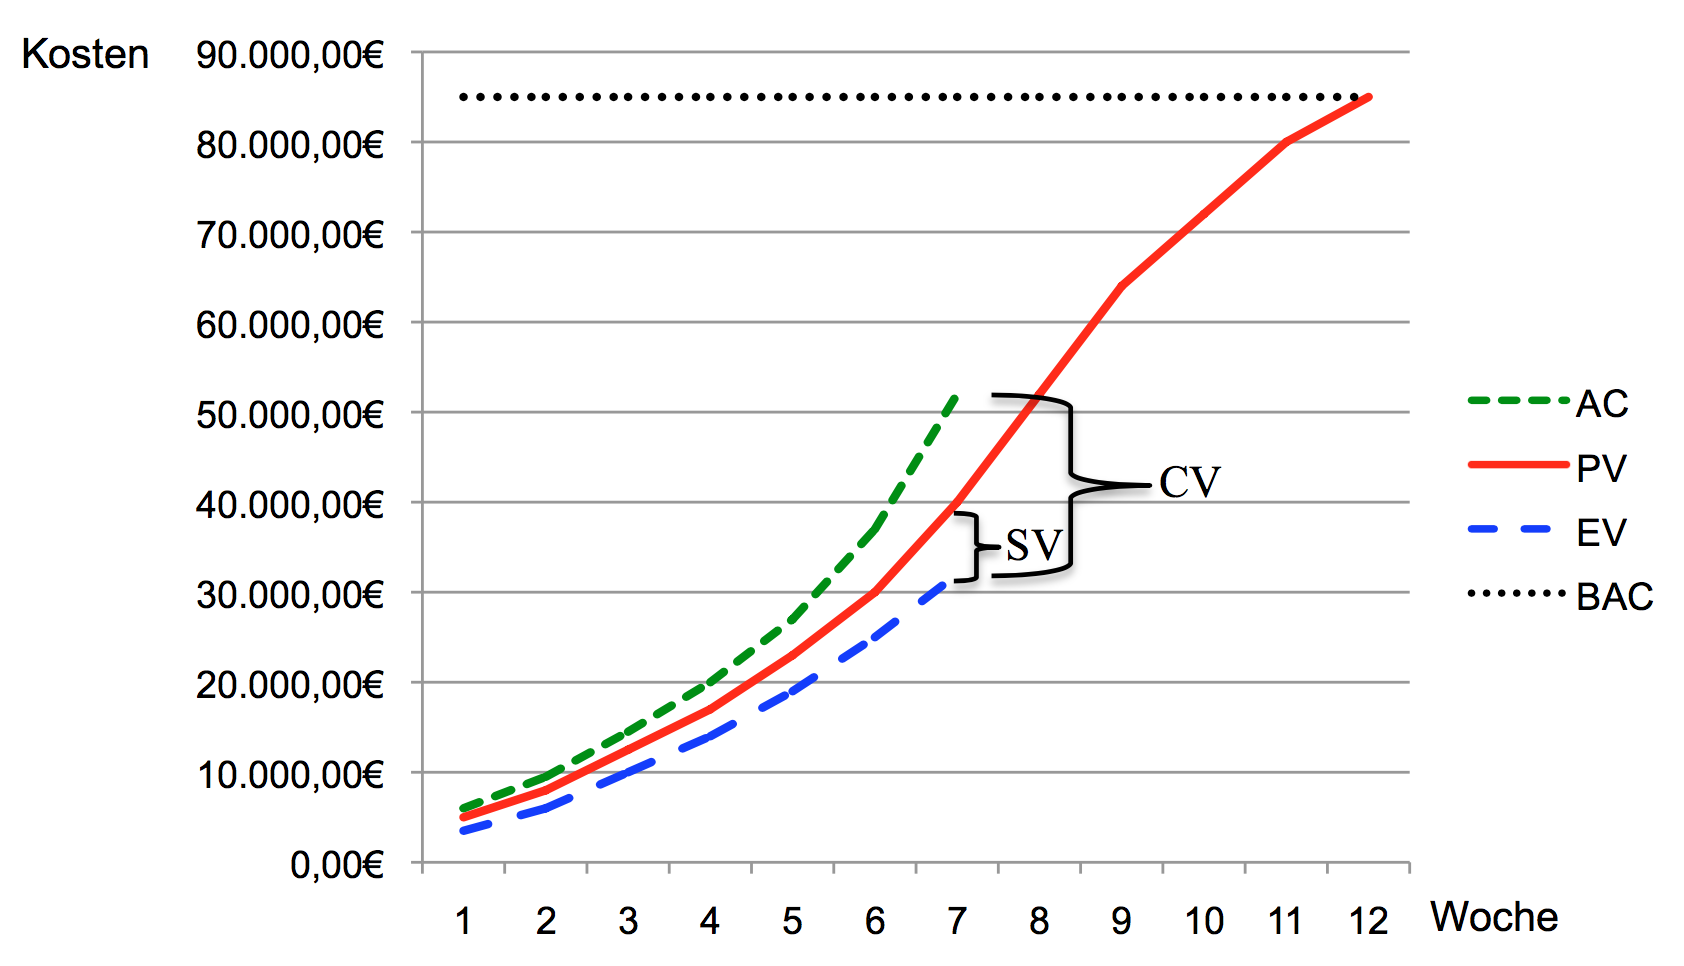
\includegraphics[width=1\textwidth,
		keepaspectratio=true]{bilder/ev_analyse.png}
\end{frame}

\begin{frame}
\frametitle{Projekt-Controlling - EVA}
	Das Projekt kann über die folgenden Leistungskennzahlen bewertet werden:
	\scriptsize
	\begin{table}[]
		\begin{tabular}{lll}
		 CPI & Cost Performance Index & CV = EV / AC \\
		 SPI & Schedule Performance Index & SV = EV / PV \\
		\end{tabular}
	\end{table}
	\normalsize
	Bei einem guten Projekt sollten beide Werte in einem schmalen und
	definiertem Intervall um 1 liegen.
	\begin{table}[]
		\begin{tabular}{ll}
		 \cellcolor[HTML]{9FD477} CPI \textgreater 1 & \cellcolor[HTML]{9FD477} Geleistete Arbeit war günstiger als geplant \\
		 \cellcolor[HTML]{FC6D58} CPI \textless 1 & \cellcolor[HTML]{FC6D58} Geleistete Arbeit war teurer als geplant \\
		 \cellcolor[HTML]{9FD477} SPI \textgreater 1 & \cellcolor[HTML]{9FD477} Es konnte mehr erreicht werden als geplant \\
		 \cellcolor[HTML]{FC6D58} SPI \textless 1 & \cellcolor[HTML]{FC6D58} Arbeitsforschritt ist geringer als geplant \\
		\end{tabular}
	\end{table}
\end{frame}

\begin{frame}
\frametitle{Projekt-Controlling - EVA}
	Beispiel: Nach 7 Monaten stellen wir bei einem Projekt die folgenden Werte fest:
	\begin{itemize}
		\item AC = 52000
		\item PV = 40000
		\item EV = 32000
		\item SPI = 0.8
		\item CPI = 0.61
	\end{itemize}
	Bis zum Berichtszeitpunkt wurde also 20 Prozent weniger Leistung erbracht als geplant.
	Da der tatsächliche Aufwand dabei höher war als geplant, liegt das Projekt 39 Prozent
	unter der Leistung die nach den Kosten zu erwarten war.
	\normalsize
\end{frame}

\begin{frame}
\frametitle{Software-Metriken}
	Software-Metriken dienen der Quantifizierung der internen Struktur eines Softwaresystems.
	Sie sind leicht zu messen, müssen jedoch mit Bedacht gewählt und berücksichtigt werden
	da Sie nicht notwendigerweise Aussagen über die Qualität treffen können.
	\scriptsize
	\begin{block}{Dynamische Metriken}
		Werden während der Ausführung des Programms gesammelt (z.B. während des Testens oder wenn
		das System produktiv genutzt wird). \\
		Beispiele: Anzahl Bugtickets des letzten Monats, Anzahl offener TCP Connections, Anzahl arbeitender Threads,
		verwendeter Heapspace, durschnittliche Round-Trip-Zeit eines Requests \ldots
	\end{block}
	\begin{block}{Statische Metriken}
		Werden aus verschiedenen Sichten / Modellen des Systems gesammelt, wie Beispielsweise Klassendiagrammen,
		dem Quellcode oder der Dokumentation.
	\end{block}
	\normalsize
	Im folgenden befassen wir uns mit statischen Softwaremetriken.
\end{frame}

\begin{frame}[fragile]
	\frametitle{Kopplung}
		\begin{itemize}
		  \item Abh\"angigkeit zwischen Klassen
		  \item Kopplung definiert Grad der Abh\"angigkeit
		  \item Zeigt Einfluss von \"Anderungen einer Klassen
		  auf andere Klassen auf
		  \item Ziel: Lose/Geringe Kopplung zwischen Klassen
		\end{itemize}
\end{frame}

\begin{frame}[fragile]
	\frametitle{Koh\"asion}
		\begin{itemize}
		  \item Grad des Zusammenhangs aller Verantwortlichkeiten, Daten und
		  Methoden einer Klasse
		  \item Ziel ist eine hohe Koh\"asion innerhalb einer Klasse/Methode\ldots
		\end{itemize}
\end{frame}

\begin{frame}[fragile]
	\frametitle{Fan-in / Fan-out}
		Fan-in
		\begin{itemize}
		  \item Anzahl der Methoden die eine andere Methode (z. B. x())  aufrufen
			\item Eine hohe Anzahl bedeutet eine starke Kopplung von x() zu den restlichen Komponenten
			\item Änderungen von x() kann tiefgreifende Folgen für das Gesamtsystem haben
		\end{itemize}
		Fan-out
		\begin{itemize}
		  \item Anzahl der Methoden die von Methode x() aufgerufen werden
			\item Eine hohe Anzhal bedeutet eine hohe Komplexität von x() da
						viel Steuerungslogik zur Koordination der Methodenaufrufe nötig ist
		\end{itemize}
\end{frame}

\begin{frame}[fragile]
	\frametitle{Lines of code (LOC)}
		\begin{itemize}
		  \item Misst die Größe des Programms anhand des Quellcodes
			\item Allgemein gilt je größer eine Komponente ist desto komplexer und fehleranfälliger ist sie
			\item Eine der zuverlässigsten Metriken zur Vorhersage fehleranfälliger Komponenten
		\end{itemize}
\end{frame}

\begin{frame}[fragile]
	\frametitle{Cyclomatic Complexity}
		\begin{itemize}
		  \item Anzahl linear unabhängiger Pfade innerhalb einer Methode
			\item Gibt die minimale Anzahl an Tests vor die benötigt werden um eine
						komplette Testabdeckung der Methode zu erzielen
			\item Mögliche Berechnung: Anzahl der Verzweigungen mit genau 2 Zweigen + 1
			\item Bei verschachtelten Verzweigungen oder Verzweigungen mit mehreren möglichen Wegen
						werden diese auf Binärverzweigungen heruntergebrochen
		\end{itemize}
\end{frame}

\begin{frame}[fragile]
	\frametitle{Length of identifiers (LOI)}
		\begin{itemize}
		  \item Durchschnittliche Länge von Variablen-, Methoden-, Klassennamen \ldots
			\item Je länger die Namen desto höher ist oftmals die Ausdrücksstärke und Verständlichkeit
						des Programms
		\end{itemize}
\end{frame}

\begin{frame}[fragile]
	\frametitle{Depth of conditional nesting}
		\begin{itemize}
		  \item Misst die Tiefe der Verzweigungen in einer Methode
			\item Sehr tiefe Verzweigungsbäume sind häufig schwer zu verstehen, fehleränfällig
						und lassen sich nur mit Seiteneffekten modifizieren
		\end{itemize}
\end{frame}

\begin{frame}[fragile]
	\frametitle{Weighted methods per class (WMC)}
		\begin{itemize}
		  \item Anzahl der Methoden einer Klasse Gewichtet nach Komplexität
			\item Einfache Methoden haben eine Komplexität von 1
			\item Komplexe Methoden können beliebig hohe Gewichtungen erhalten
			\item Je höher der Wert der Metrik desto komplexer ist die Gesamtstruktur der Klasse
			\item Oftmals sind komplexe Klassenstrukturen gering Kohäsiv und schwer wiederverwendbar
		\end{itemize}
\end{frame}

\begin{frame}[fragile]
	\frametitle{Depth of inheritance tree (DIT)}
		\begin{itemize}
		  \item Anzahl der Stufen in einem Vererbungsbaum in dem eine Kindklasse die Attribute und Operationen
						der Vaterklasse erbt
			\item Je tiefer der Baum desto komplexer die Komponente
			\item Das Nutzen der Blätter (tiefsten Kindklassen) setzt das Verständis einer hohen Anzahl von Vaterklassen voraus
		\end{itemize}
\end{frame}

\begin{frame}[fragile]
	\frametitle{Number of children (NOC)}
		\begin{itemize}
		  \item Misst die Anzahl der direkten Kindklassen einer Vaterklasse
			\item NOC misst die Breite einer Klassenhierarchie während DIT die Tiefe misst
			\item Ein hoher Wert gilt als Indikator für hohe Wiederverwendung
		\end{itemize}
\end{frame}
